\documentclass{article}
\usepackage{graphicx} % Required for inserting images
\usepackage{biblatex}
\addbibresource{refs.bib}
\usepackage{amsmath}

\title{AST9051SP - Statistical Methods in Computational Cosmology}
\author{Metin San}
\date{April 2024}

\begin{document}

\maketitle

\section*{Project description}
This document is the final report for the project in the course AST9051SP - Statistical Methods in Computational Cosmology.
In this project, we have explored the process of fitting two non-linear parameters in a model through linear and Bayesian methods.
This document is accompanied by a Jupyter notebook where we solve a subset of the exercises in the Data analysis recipe: Fitting a model to data\cite{hogg}. The source code repository containing the code used to produce the results in this document is available at \url{https://www.github.com/metinsa/}.


\section*{Introduction}
\begin{figure}[ht]
    \centering
    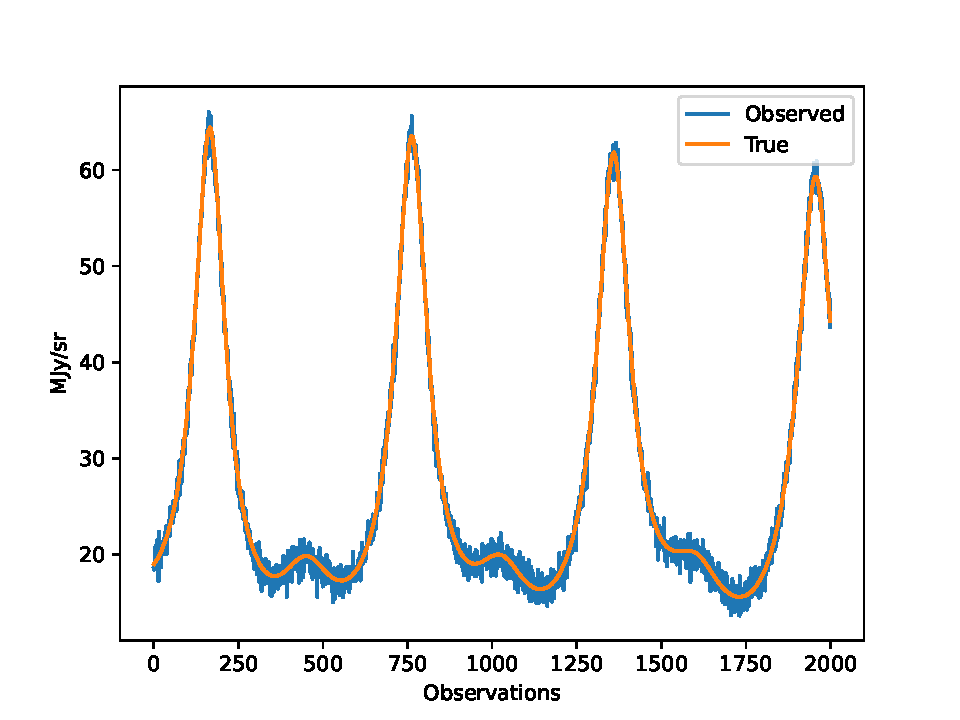
\includegraphics[width=0.9\textwidth]{figs/timestream.pdf}
    \caption{A small subsection of the data worked with in this project. The orange curve is the simulated $z_t$ timestream with ZodiPy, and the blue curve is data stream $d$ where we have added noise.}
    \label{fig:data}
\end{figure}
We will now attempt to fit the two non-linear parameters ($\alpha$, $\gamma$) in the state-of-the-art COBE/DIRBE zodiacal light model\cite{Kelsall1998}. Zodiacal light (ZL) is scattered and re-emitted sunlight by interplanetary dust in the Solar system. In the following, we will fit this model to a data stream containing ZL simulated with ZodiPy\cite{San2022, San2024} and white noise. For simplicity, the simulated ZL only contains the smooth component (diffuse cloud component) of the zodiacal cloud. This data stream represents the observed emission by the COBE/DIRBE experiment at $12 \mu$m during DIRBE observational days 50-59. A small subsection of the simulated data is shown in Figure \ref{fig:data}. The true parameter values used to generate this data are $\theta_\mathrm{true} = (\alpha_\mathrm{true}, \gamma_\mathrm{true}) = (1.337, 0.942)$.

The data model is given as
\begin{equation}
    d_t = z_t + n,
\end{equation}
where $z_t$ is the simulated ZL timestream, and $n \sim \mathcal{N}(0, 1)$. The ZL $z_t$ is proportional to the line-of-sight integral over the number density of interplanetary dust (IPD) grains $n$ multiplied by the Planck function $B_\lambda$
\begin{equation}\label{eq:zt}
    z_t \propto \int n(s) B_\lambda ds,
\end{equation}
where $s$ is the line-of-sight. The two parameters we want to fit is contained in the expression of the heliocentric ecliptic IPD number density $n(x,y,z)$, which is given as
\begin{equation}\label{eq:n}
    n(x,y,z) = n_0 r^{-\alpha} e^{ -\beta g^{\gamma}},
\end{equation}
where $n_0$ is the density of the IPD at 1 AU, $r$ is the radial distance from the origin of the IPD, and $\alpha$ and $\gamma$, the parameters we wish to fit, are shape parameters describing the radial and vertical distribution of the dust.
Furthermore we have
\begin{equation}\label{eq:g}
    g = \begin{cases}
        \zeta^2 / 2\mu & \text{for }  \zeta < \mu \\
        \zeta - \mu/2 & \text{for }  \zeta \geq \mu ,\\
    \end{cases}
\end{equation}
where $\zeta = |Z|/r$ and $Z$ is the height above the symmetry plane of the dust. When fitting our parameters we will have to fit evaluate Eq. \eqref{eq:zt}. For this purpose we use a modified version of the ZodiPy code available at the repository link at the top of this document.

We start by building some intuition over how these two parameters affect the timestream by evaluating the model over a range of these parameters. The results are shown in Fig. \ref{fig:params}. We observe that these parameters mostly affect the shape of the dips and not so much the peaks.
\begin{figure}
    \centering
    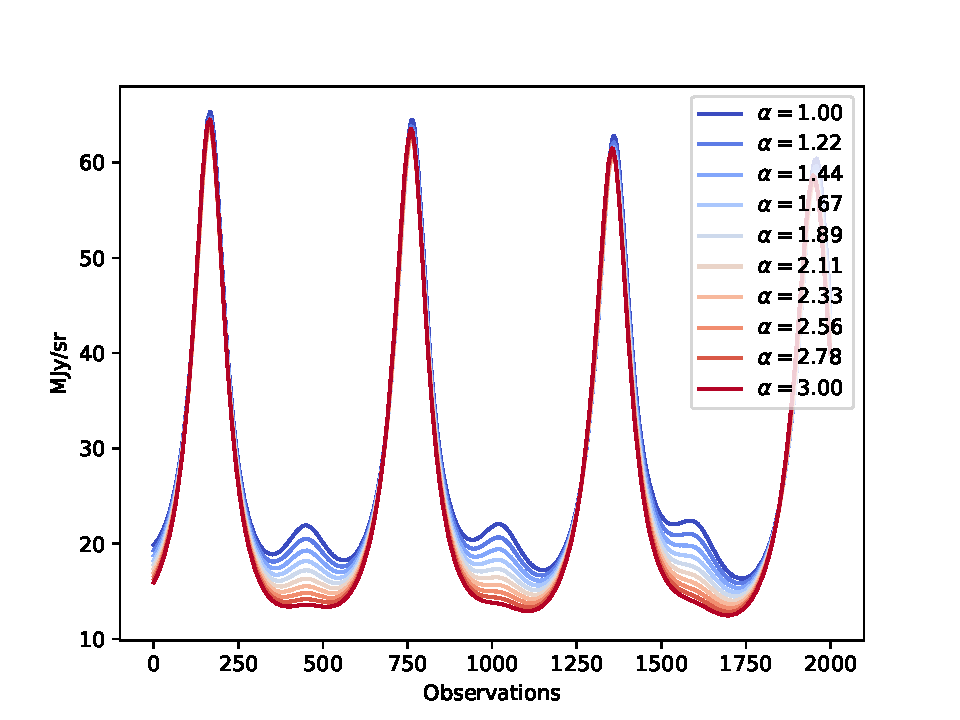
\includegraphics[width=0.9\textwidth]{figs/alpha.pdf}
    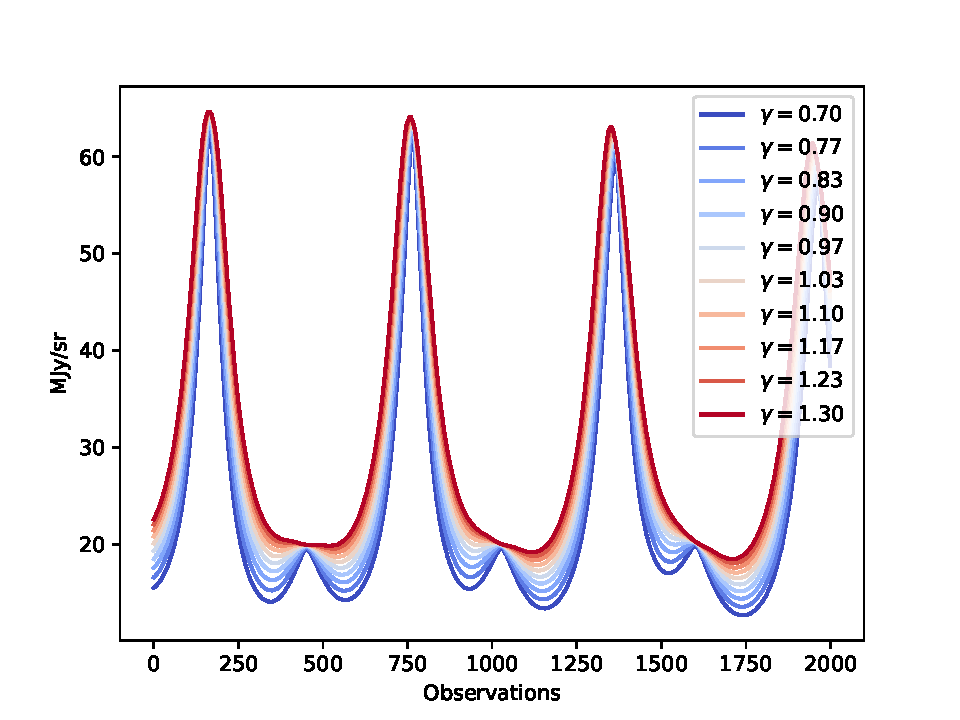
\includegraphics[width=0.9\textwidth]{figs/gamma.pdf}
    \caption{The effect of varying the two parameters $\alpha$ and $\gamma$ on the timestream, shown in the top and bottom panels respectively.}
    \label{fig:params}
\end{figure}

In order to compare two models we need a statistical quantity that measures how well our model reproduces the data. For this purpose we will use the $\chi_2$ statistic, given by
\begin{equation}
\chi^2 = \sum_i^N \frac{\left( y_i - \hat{y_i}\right)^2}{\sigma_{y, i}^2},
\end{equation}
where $y_i$ is the observed data, $\hat{y}_i$ is the prediction made by out model with parameters $\theta = (\alpha, \gamma)$, and $\sigma_{y, i}$ is the uncertainties associated with $y_i$. Since our $y_i$ values come from simulated data with noise drawn independently from a normal distribution with mean 0 and variance 1 the $\chi^2$ reduces to
\begin{equation}\label{eq:chisq}
\chi^2 = \sum_i^N \left( y_i - \hat{y_i}\right)^2.
\end{equation}
The loglikelihood in our case, which we will use when sampling the parameters, is then simply
\begin{equation}
    \mathcal{L} = -\frac{1}{2}\chi^2.
\end{equation}

\section*{Grid search}
Since we are only working two parameters it is perfectly possible to do a grid search over the parameter space to find the best fit. This is when we evaluate our model for $z_t$ over a grid of $\theta$ values and record the chisq. We note that the volume of the parameter space grows exponentially with the number of parameters, and grid searches are therefore not feasible for high-dimensional parameter spaces. In these cases we can use more advanced methods such as Markov Chain Monte Carlo (MCMC) methods, which we will do in the next section. These methods also lets us characterize the uncertianties in the parameters, unlike the grid method which simply lets us find the maximum likelihoods.

We evaluating the model over a grid of $50 \times 50$ points with parameters ranging from $\alpha \in (1, 1.6)$ and $\gamma \in (0.6, 1.2)$. The resulting $\chi^2$ values are shown in in Figure \ref{fig:grid}. From the eliptical shape of the $\chi^2$ values we can see that the two parameters are indeed correlated, which is also what we see in the model plots in Figure \ref{fig:params}.

\begin{figure}
    \centering
    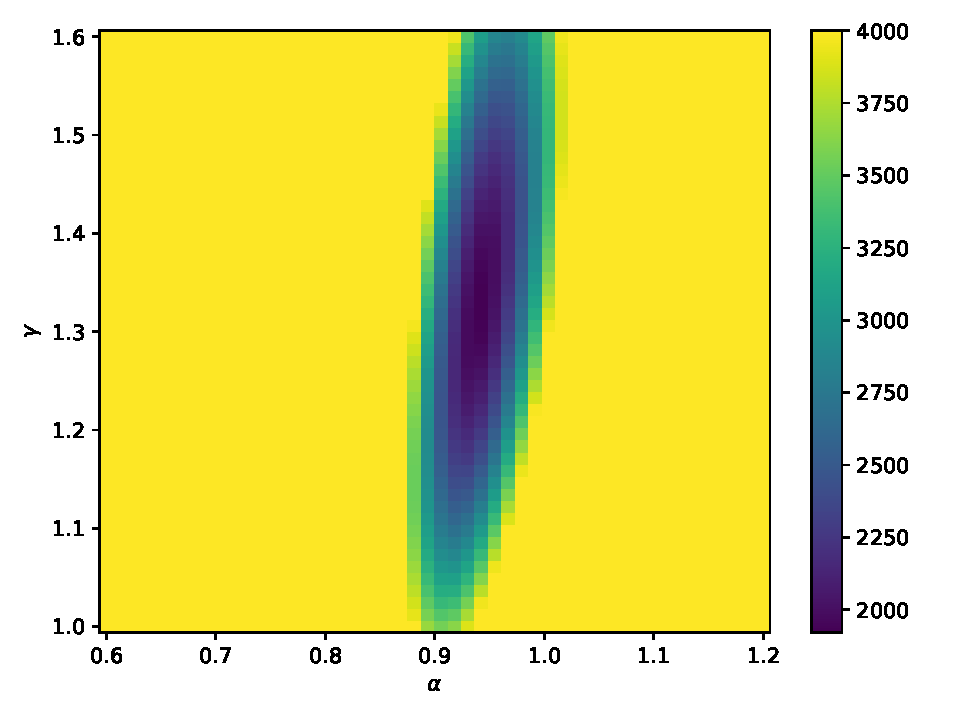
\includegraphics[width=0.9\textwidth]{figs/grid_chisq.pdf}
    \caption{The $\chi^2$ values for the grid search over the parameter space.}
    \label{fig:grid}
\end{figure}


\section{Metropolis-Hastings}
The next method we will use to sample these parameters is the Markov Chain Monte Carlo (MCMC) Metropolis-Hastings algorithm.
Metropolis-Hastings lets us sample from a generic probability distribution $P(\theta)$ even when we don't know the true underlying distribution. It works by iterativly accepting or rejecting candidate samples from a target distribution $g(\theta) \propto P(\theta)$. The algorithm is described below

\begin{enumerate}
    \item Select an initial value $\theta_0$
    \item for i = 1, ..., n, repeat:
    \begin{enumerate}
        \item Draw a candidate $\theta^* \sim q(\theta^* | \theta_{i-1})$ from the proposal distribution $q$
        \item Compute the acceptance factor $a$ (usually $\alpha$ but we already used $\alpha$ for the fitted parameter)
        \begin{equation}
            a = \frac{g(\theta^*)/q(\theta^* | \theta_{i-1})}{g(\theta_{i-1})/q(\theta_{i-1} | \theta^*)} = \frac{g(\theta^*) q(\theta_{i-1} | \theta^*)}{g(\theta_{i-1}) q(\theta^* | \theta_{i-1})}
        \end{equation}
        
        \item if $a \geq 1$: accept $\theta^*$ and set $\theta_i \leftarrow \theta^*$

        if $0 < a < 1 $ accept $\theta^*$ and set $\theta_i \leftarrow \theta^*$ with probability $a$

        else: reject $\theta^*$ and set $\theta_i \leftarrow \theta_{i-1}$ with probability $1 - a$.
    \end{enumerate}
\end{enumerate}
We will draw the candidate $\theta^*$ from a normal distribution $\mathcal{N}(\theta_{i-1}, \mathrm{const})$. Since the normal distribution is symmetric about its mean, the ratio of the proposal distributions $q(\theta^* | \theta_{i-1})/q(\theta_{i-1} | \theta^*)$ cancels out, leaving us with the so called random walk Metropolis Hasting with 
\begin{equation}
    a = \frac{g(\theta^*)}{g(\theta_{i-1})}.
\end{equation}
The target distribution in our case is 
\begin{equation}
    g(\theta) = \mathrm{const} \exp\left[-\frac{1}{2}\chi^2\right],
\end{equation}
and 
\begin{equation}
    a = \exp \left[ {\chi^*}^2 - \chi^2_{i-1}\right],
\end{equation}
where we get the $\chi^2$ by evaluating the ZodiPy model for the candidate $\theta$ values similarly to in the grid search case. 

We select initial values $\theta_0 = (\alpha_0, \gamma_0) = (1.2, 0.92)$. Additionally, we need to select stepsizes $\Delta_\theta$ which we use to draw the candidate samples. We pick these to be $\Delta_\theta = (\Delta_\alpha, \Delta_\gamma) = (0.01, 0.005)$, motived by the values from the $\chi^2$ grid. We let the Metropolis-Hastings algorithm run for 10000 iterations, and make three trace plots: 1) A trace plot of $\alpha$, $\gamma$, and $\chi^2$ for all 10000 samples, 2) A trace plot of the same parameters but with the first 1000 samples removed (burn-in phase), and 3) A corner plot showing the correlation between the two parameters. The results are shown in Figures \ref{fig:mh}, \ref{fig:mh_burnin}, and \ref{fig:mh_corner}.
\begin{figure}
    \centering
    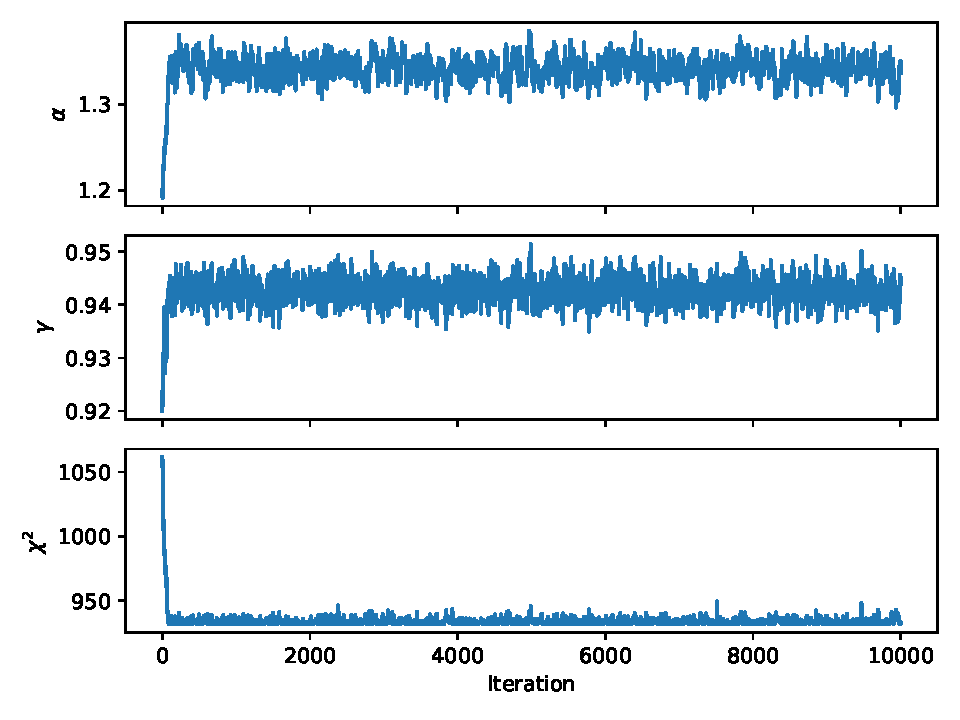
\includegraphics[width=0.9\textwidth]{figs/mh.pdf}
    \caption{Trace plot showing 10000 samples (including the burn-in phase) of the parameters $\alpha$, $\gamma$, and the $\chi^2$ metric, using the Metrpolis-Hasting algorithm.}
    \label{fig:mh}
\end{figure}
\begin{figure}
    \centering
    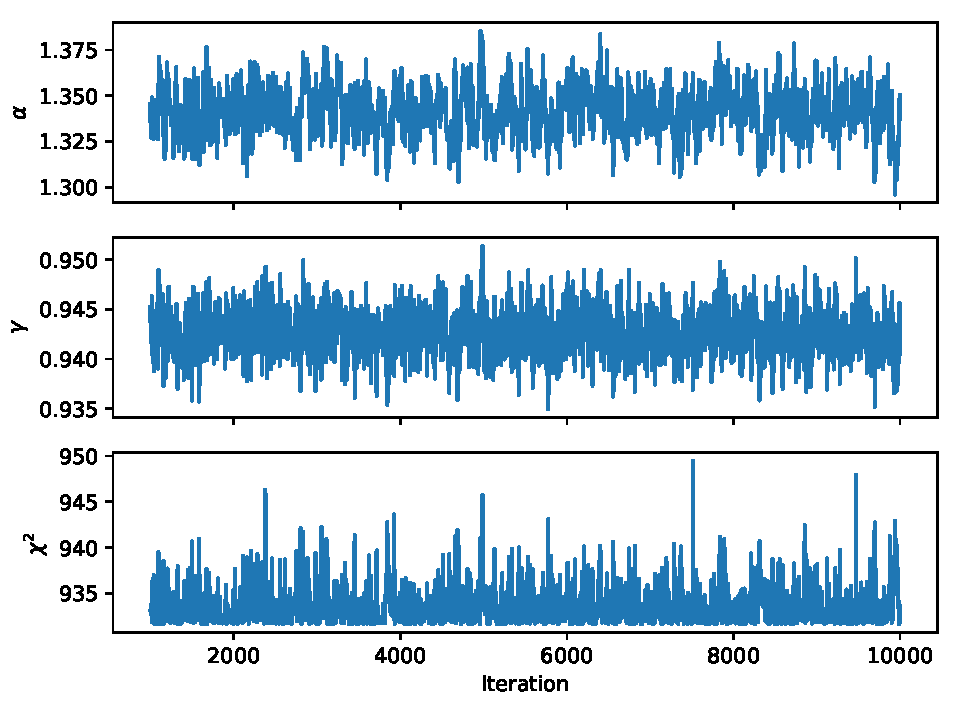
\includegraphics[width=0.9\textwidth]{figs/mh_postburnin.pdf}
    \caption{Trace plot showing 9000 samples of the parameters $\alpha$, $\gamma$, and the $\chi^2$ metric, using the Metrpolis-Hasting algorithm.}
    \label{fig:mh_burnin}
\end{figure}
\begin{figure}
    \centering
    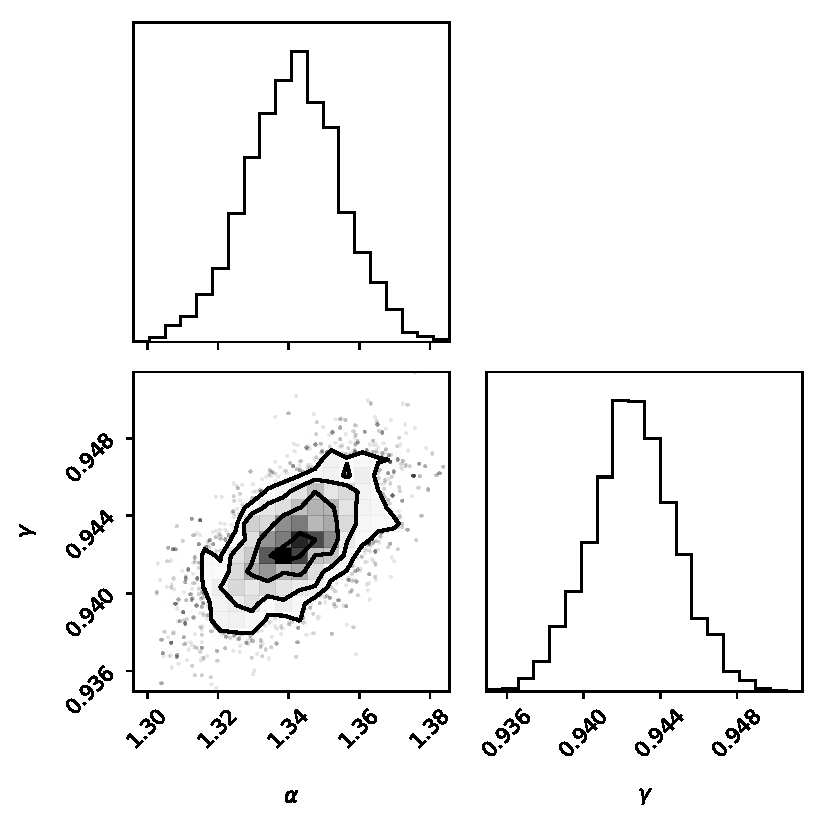
\includegraphics[width=0.9\textwidth]{figs/mh_corner.pdf}
    \caption{Corner plot showing the 1- and 2-D histograms and the parameters $\alpha$, $\gamma$, obtained from post burn-in Metropolis Hastings samples.}
    \label{fig:mh_corner}
\end{figure}

We can find the maximum likelihoods of the parameters by finding the sample with the smallest $\chi^2$ value
\begin{equation}
    \theta_\mathrm{ML} = \theta[\mathrm{argmin}(\chi^2)].
\end{equation}
However, there are other quicker ways to estimate the maximum likelihoods. The main benefit of the MCMC method is that it lets us estimate the uncertainties in the parameters, which is otherwise traditional difficult to estimate. We can compute the mean and standard deviation of the parameters from the chain as follows
\begin{align}
    \mu_\theta &= \frac{1}{N} \sum_i^N \theta_i,\\
    \sigma_\theta^2 &= \frac{1}{N} \sum_i^N (x_\theta - \mu_\theta)^2.
\end{align}
We find that for 9000 samples with an accept rate of 0.3405\%, the best fit parameters using Metropolis-Hastings are
\begin{align*}
    \alpha &= 1.3420 \pm  0.0155\\
    \gamma &= 0.9426 \pm  0.0024.
\end{align*}

\section{Hamiltonian Monte Carlo}
Although the Metropolis-Hastings seems to do a good job at sampling the parameters in our case, it can be very inefficient in exploring the full parameter space and may sometimes lead to slow convergence. Another sampling method, which required much fewer samples to converge is the Hamiltonian Monte Carlo method (HMC). HMC is very similar to Metropolis-Hastings in that we propose a new sample and either accept or reject with some probability. But rather than taking random steps in the parameter space, we instead use Hamiltonian dynamics to find the new proposals. This allows us to move to distant states with high probability of acceptance due to the energy conserving properties of the Hamiltonian. The Hamiltonian is given as
\begin{equation}
H(q, p) = K(p) + V(q),
\end{equation}
where $K(p, q)$ is the kinetic energy which depends on the momentum $p$,
\begin{equation}
    K(p) = \frac{1}{2}p^2,
\end{equation}
and the $V(q)$ is the potential energy. The trick to using the Hamiltonian in a MCMC context is that we set the position equal to the parameters we wish to fit $q \equiv \theta$, and set the potential $V$ to the negative log likelihood of our target distribution
\begin{equation}
    V(\theta) = \log \mathcal{L}(\theta) = -\frac{1}{2}\chi^2.
\end{equation}
This allows us find new parameter samples by solving the equations of motion and moving in parameter space along equal energy curves. At any given position $\theta_i$, we can draw a random value for the momentum $p$, and integrate the Hamiltonian to move along equal energy curves in phase space to pick a new value for parameter value $\theta_{i+1}$ with much higher acceptance probability than in the random walk Metropolis-Hastings scenario. The accept rate for MHC is analogous to Metropolis-Hastings
\begin{equation}
    a = \mathrm{min} \left(1, \exp \left( H(\theta_i, p_i) - H(\theta_{i+1}, p_{i+1})\right) \right).
\end{equation}

A volume conserving numerical integration technique is required to to integrate the Hamiltonian. The most commonly used algorithm is the Leap frog algorithm, which is similar to Euler's method, but instead of taking a full step at each iteration, it first takes half a step in momentum $p_{i+1/2}$ and then uses that to find $q_{i+1}$ and $p_{i+1}$ in a volume or energy conserving way:
\begin{align}
    p_{i+1/2} &= p_i + \frac{\epsilon}{2} \nabla_\theta V(\theta_i)\\
    \theta_{i+1} &= \theta_i + p_{i+1/2} \frac{\epsilon}{2}\\
    p_{i+1} &= p_{i+1/2} + \frac{\epsilon}{2} \nabla_\theta V(\theta_{i+1}),\\
\end{align}
where $\epsilon$ is the a step size and $\nabla_\theta V(\theta)$ is the gradient of the potential energy, or in our case, the log-likelihood. This is where we see one of the downside of HMC - it requires us to know the $\nabla_\theta V(\theta)$, the gradient of the log likelihood
\begin{equation}
\nabla_\theta = \sum \left[y - \hat{y}(\theta)\right] \frac{\partial \hat{y}(\theta)}{\partial \theta}.
\end{equation}
For us that amounts to two new functions that we need to compute by differentiating Eq \eqref{eq:n} with respect to $\alpha$ and $\gamma$

\begin{align}
    \frac{\partial n}{\partial\alpha}
    &=-n_0 r^{-\alpha}f\ln r
    =-n\ln r\\
    \frac{\partial n}{\partial \gamma}
    &=n_0 r^{-\alpha} f(-\beta g^\gamma \ln g)
    =-\beta g^\gamma\ln g \; n
\end{align}

\begin{figure}
    \centering
    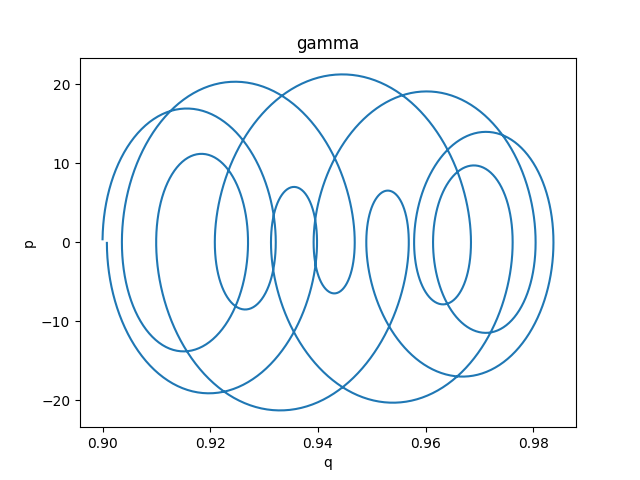
\includegraphics[width=0.9\textwidth]{figs/gamma_curve.png}
    \caption{Illustrating an equal energy curve for the parameter $\gamma$.}
    \label{fig:energy curves}
\end{figure}
Figure \ref{fig:energy curves} illustrates the equal energy phase space contours that we move along for the parameter $\gamma$ after drawing a random momentum $p$.
When selecting a new sample, we specify the two hyper parameters $L$, the number of leap-frog "leap"/iterations, and $\epsilon$. For our two parameters, we pick $L=5$, and $\epsilon=0.0001$. For each iteration, we need to additionally evaluate ZodiPy $L$ times where we also compute the gradients in Eq. (24, 25). By selecting $L=10$, $\epsilon=0.001$, and running for 5000 iterations, with an accept rate of 0.6599\% we get the following results seen in Figures \ref{fig:hmc}, \ref{fig:hmc_burnin}, and \ref{fig:hmc_corner}. The best fit parameters from these chains are
\begin{align*}
    \alpha &= 1.3371 \pm  0.0106\\
    \gamma &= 0.9421 \pm  0.0018.
\end{align*}
The HMC solution perfectly reproduces the underlying true parameters, with smaller uncertainties than those in the Metropolis-Hasting even with only half the samples.


\begin{figure}
    \centering
    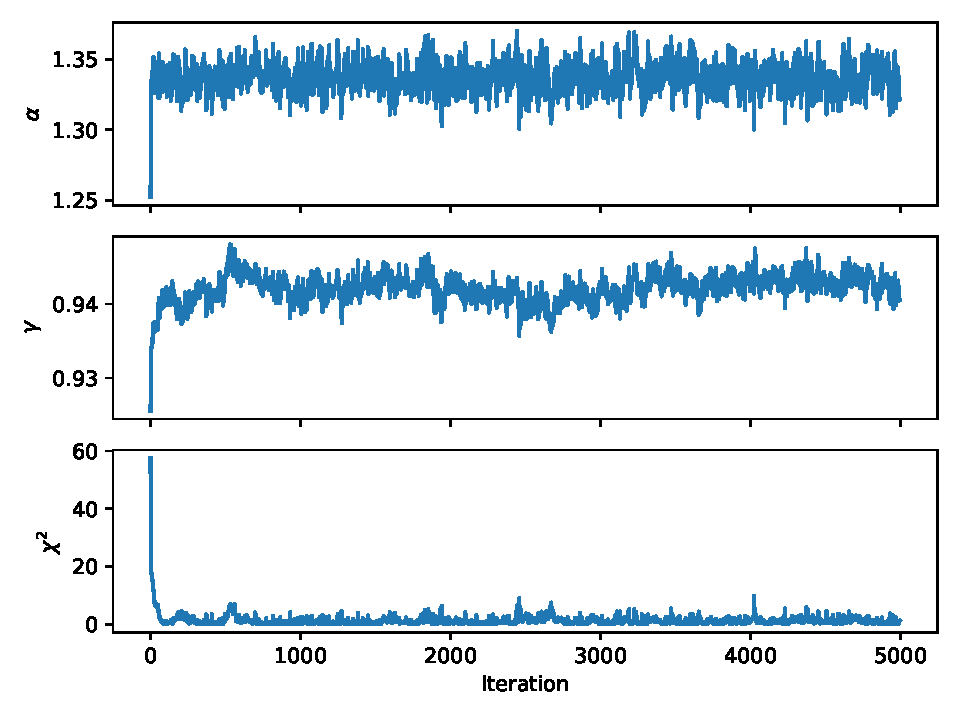
\includegraphics[width=0.9\textwidth]{figs/hmc.pdf}
    \caption{Trace plot showing 10000 samples (including the burn-in phase) of the parameters $\alpha$, $\gamma$, and the $\chi^2$ metric, using the Hamiltonian Monte Carlo algorithm.}
    \label{fig:hmc}
\end{figure}
\begin{figure}
    \centering
    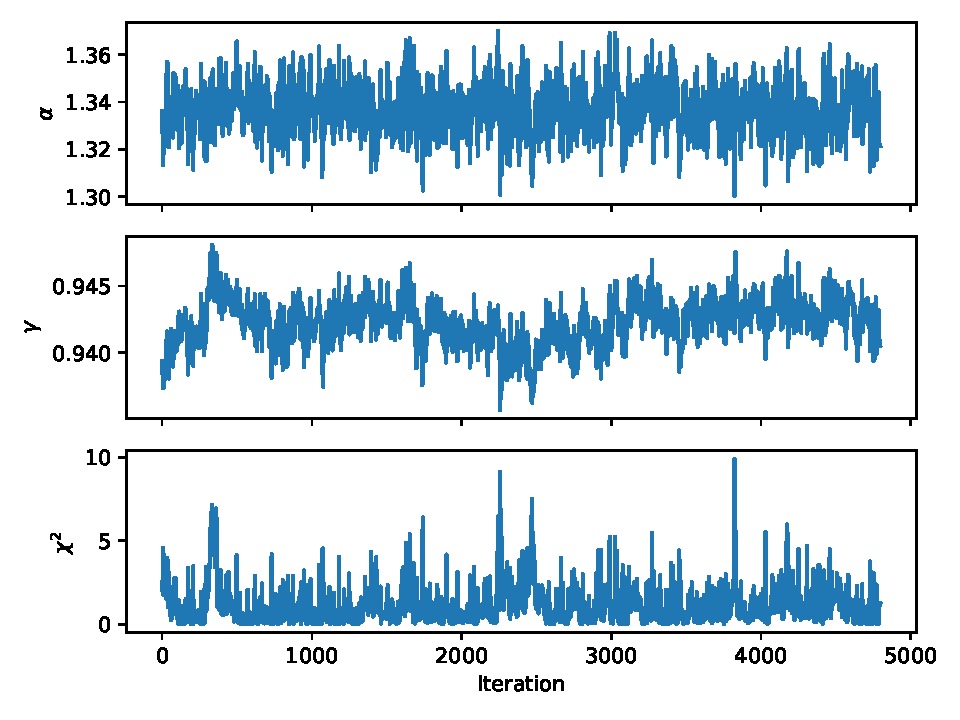
\includegraphics[width=0.9\textwidth]{figs/hmc_burnin.pdf}
    \caption{Trace plot showing 9000 samples of the parameters $\alpha$, $\gamma$, and the $\chi^2$ metric, using the Hamiltonian Monte Carlo algorithm.}
    \label{fig:hmc_burnin}
\end{figure}
\begin{figure}
    \centering
    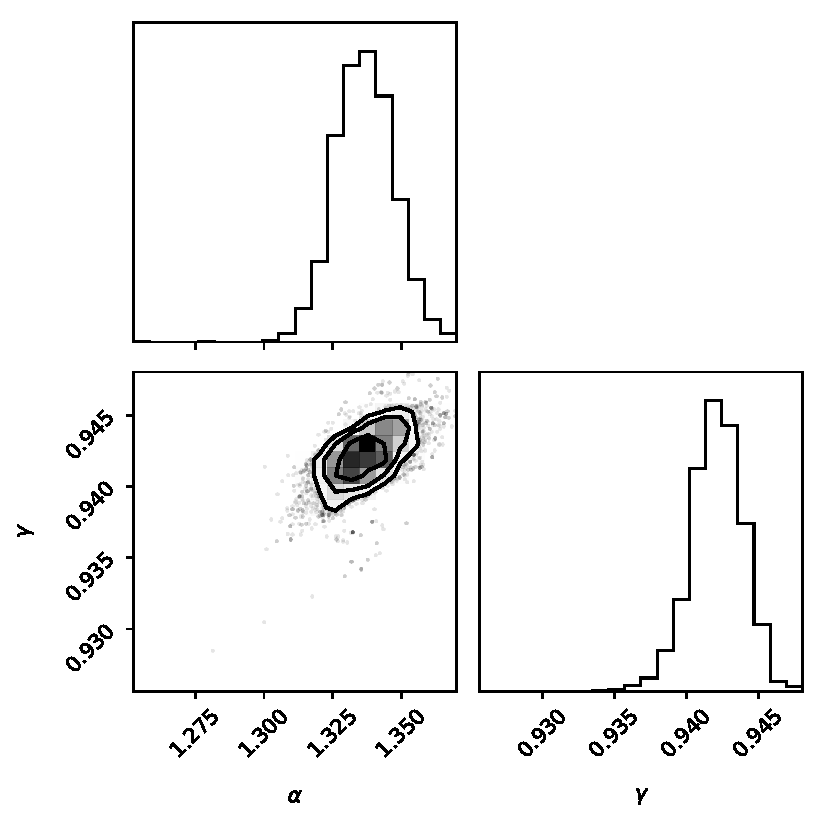
\includegraphics[width=0.9\textwidth]{figs/hmc_corner.pdf}
    \caption{Corner plot showing the 1- and 2-D histograms and the parameters $\alpha$, $\gamma$, obtained from post burn-in Hamiltonian Monte Carlo samples.}
    \label{fig:hmc_corner}
\end{figure}

\printbibliography
\end{document}